
\section{Model and Design}
\label{sec:model}


\begin{figure}[htb]
	\centering
	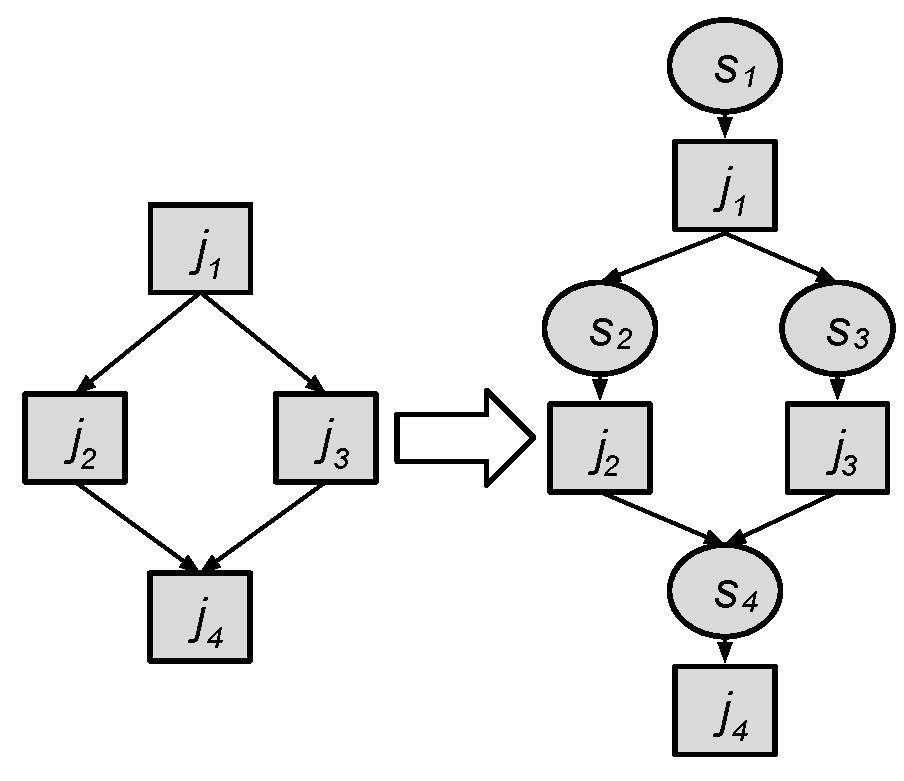
\includegraphics[width=0.7\linewidth]{figure/odag.pdf}
	\captionof{figure}{Extending DAG to o-DAG.}
	\label{fig:odag}
	\vspace{-10pt}
\end{figure}
A workflow is modeled as a Directed Acyclic Graph (DAG) as shown in \ref{fig:odag}. Each node in the DAG often represents a workflow job ($j$), and the edges represent dependencies between the jobs that constrain the order in which the jobs are executed. Dependencies typically represent data-flow dependencies in the application, where the output files produced by one job are used as inputs of another job. Each job is a single execution unit and it may contains one or multiple tasks, which is a program and a set of parameters that need to be executed. Fig.~\ref{fig:odag} (left) shows an illustration of a DAG composed by four jobs. This model fits several workflow management systems such as Pegasus~\cite{Deelman2005}, Askalon~\cite{Fahringer2005}, and Taverna~\cite{Oinn:2006:TLC:1148437.1148448}.

%Change it with job wrapper
Fig.~\ref{fig:system} shows a typical workflow execution environment. The submit host prepares a workflow for execution (clustering, mapping, etc.), and worker nodes, at an execution site, execute jobs individually. The main components are introduced below:

\begin{figure}[htb]
\centering
  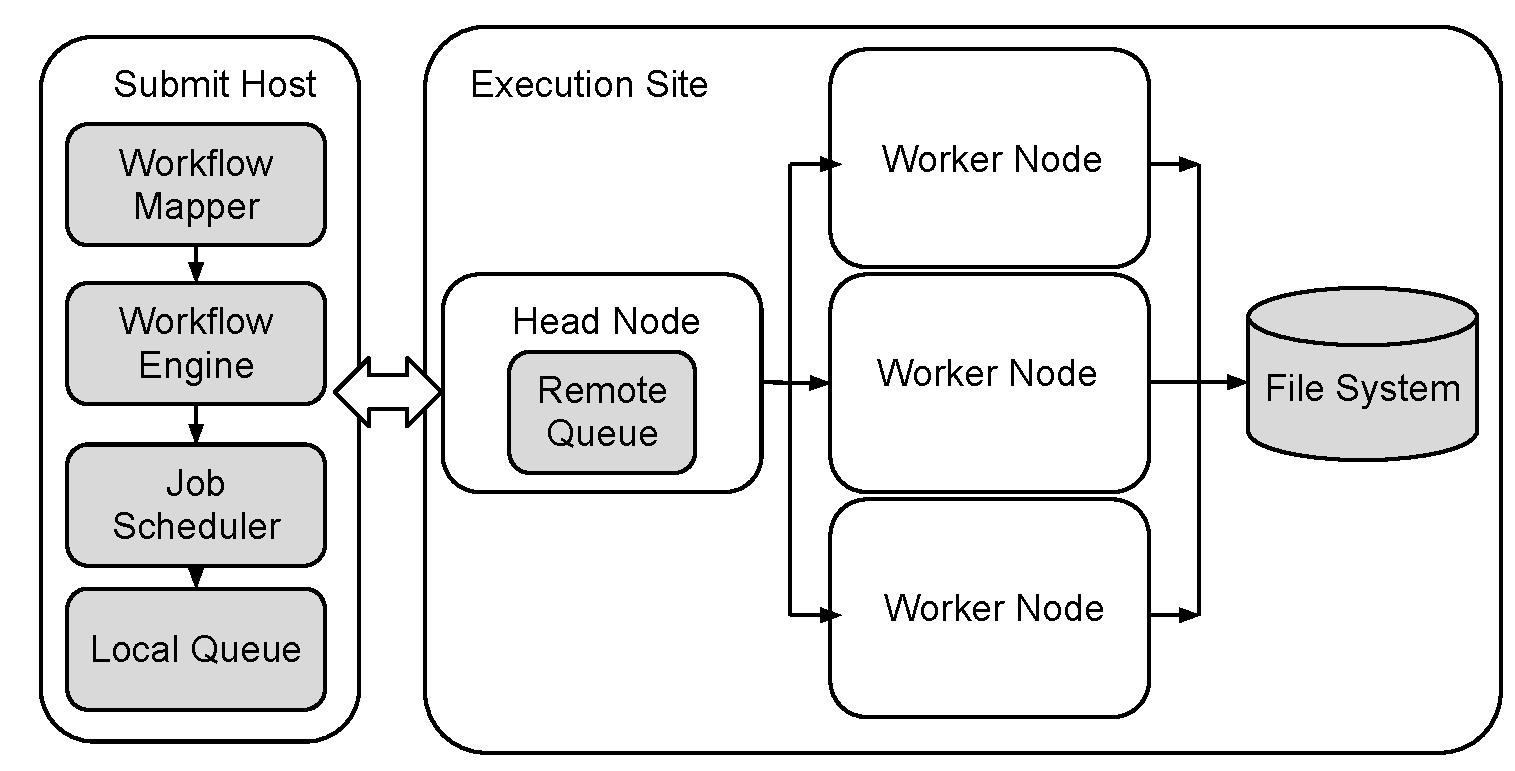
\includegraphics[width=0.95\linewidth]{figure/execution.pdf}
  \caption{A workflow system model.}
  \label{fig:system}
  \vspace{-10pt}
\end{figure}

\paragraph{Workflow Mapper} generates an executable workflow based on an abstract workflow provided by the user or work- flow composition system. It also restructures the workflow to optimize performance and adds tasks for data management and provenance information generation. In this work, workflow mapper is particularly used to merge small tasks together into a job such that system overheads are reduced, which is called Task Clustering. A job is a single execution unit in the workflow execution systems and it may contain one or more tasks.

\paragraph{Workflow Engine} executes jobs defined by the workflow in order of their dependencies. Only jobs that have all their parent jobs completed are submitted to the Job Scheduler. Workflow Engine relies on the resources (compute, storage, and network) defined in the executable workflow to perform the necessary actions. The time period when a job is free (all of its parents have completed successfully) to when it is submitted to the job scheduler is denoted the workflow engine delay. The workflow engine delay is usually configured by users to assure that the entire workflow scheduling and execution system is not overloaded. 

\paragraph{Job Wrapper} extracts tasks from clustered jobs and executes them at the worker nodes. The clustering delay is the elapsed time on the extraction process.



\paragraph{Job Scheduler and Local Queue} manage individual workflow jobs and supervise their execution on local and remote resources. The time period when a job is submitted to the job scheduler to when the job starts its execution in a worker node is denoted the queue delay. It reflects both the efficiency of the job scheduler and the resource availability. 


\begin{figure}[h!]
	\centering
    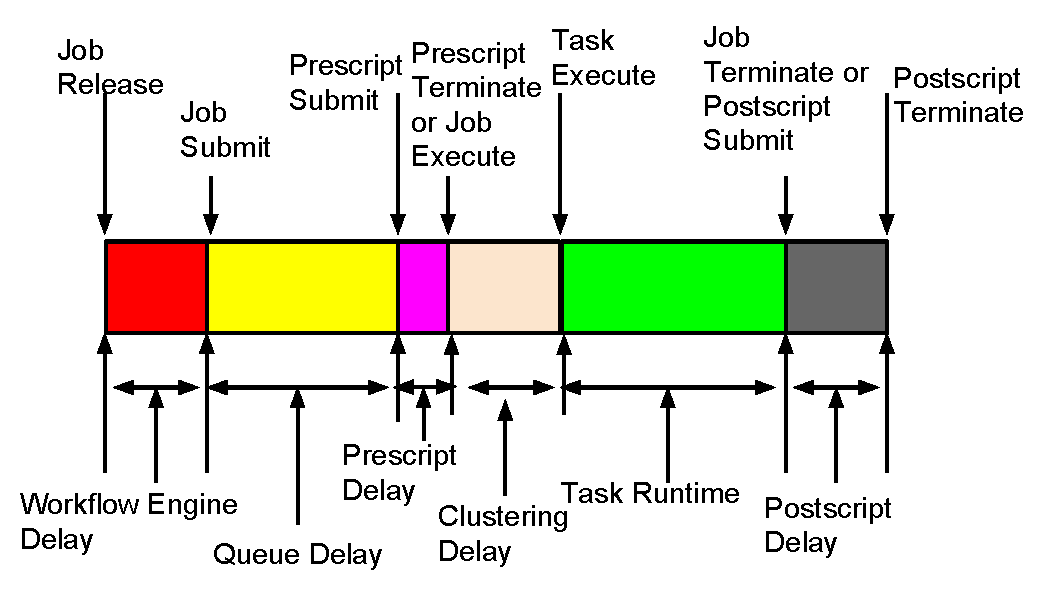
\includegraphics[width=0.5\textwidth]{figures/model/overhead.pdf}
    \caption{Workflow Events}
    \label{fig:model_overhead}
\end{figure}


The execution of a job is comprised of a series of events as shown in Figure~\ref{fig:model_overhead} and they are defined as:

\begin{enumerate}
\item Job Release is defined as the time when the workflow engine identifies that a job is ready to be submitted (when its parents have successfully completed). 
\item Job Submit is defined as the time when the workflow engine submits a job to the local queue. 
\item Job Execute is defined as the time when the workflow engine sees a job is being executed. 
\item Task Execute is defined as the time when the job wrapper sees a task is being executed. 
\item Pre/Postscript Start is defined as the time when the workflow engine starts to execute a pre/postscript. 
\item Pre/Postscript Terminate is defined as the time when the pre/postscript returns a status code (success or failure). 
\end{enumerate}

Figure~\ref{fig:overhead} shows a typical timeline of overheads and runtime in a compute job. We do not specify the data transfer delay in this timeline because data transfer is handled by data transfer jobs (stage-in and stage-out jobs). 

As shown in our prior work \cite{Chen}, we have classified workflow overheads into three categories as follows. 
\begin{enumerate}

\item{Workflow Engine Delay} measures the time between when the last parent job of a job completes and the time when the job gets submitted to the local queue. The completion time of the last parent job means this job is released to the ready queue and is waiting for resources to be assigned to it. The workflow engine delay reflects the efficiency of a workflow engine (i.e., DAGMan~\cite{DAGMan}). 

\item{Queue Delay} is defined as the time between the submission of a job by the workflow engine to the local queue and the time the local scheduler sees the job running. This overhead reflects the efficiency of the local workflow scheduler (e.g. Condor \cite{Frey2002}) to execute a job and the availability of resources for the execution of this job. 

\item{Pre/Postscript Delay } is the time taken to execute a lightweight script under some execution systems before/after the execution of a job. For example, prescripts prepare working environment before the execution of a job starts and postscripts examine the status code of a job after the computational part of this job is done.

\item{Clustering Delay} measures the difference between the sum of the actual task runtime and the job runtime seen by the job wrapper. The cause of Clustering Delay is usually because we use a job wrapper in worker nodes to execute a clustered job that requires some delay to extract the list of tasks. 

\end{enumerate}

The overhead aware DAG model (o-DAG) we use in this work is an extension of the traditional DAG model. System overheads play an important role in workflow execution and constitute a major part of the overall runtime when jobs are poorly mapped to resources. Fig.~\ref{fig:odag} shows how we augment a DAG to be an o-DAG with the capability to represent system overheads ($s$) such as workflow engine delay and queue delay.  


In summary, an o-DAG representation allows the specification of high level system overhead details, which is more suitable for the study of overhead aware scheduling. 

%Need to fix this
With an o-DAG model, we can explicitly express the process of task clustering. For instance, in Fig. 3, two tasks t1 and t2, without data dependency between them, are merged into a clustered job j1. A job j is a single execution unit composed by one or multiple task(s). Job wrappers are commonly used to execute clustered jobs, but they add a overhead denoted the clustering delay c. Clustering delay measures the difference between the sum of the actual task runtimes and the job runtime seen by the job scheduler. After horizontal clustering, t1 and t2 in j1 can be executed in sequence or in parallel, if supported. In this paper, we consider sequential executions only. Given a single resource, the overall runtime for the workflow in Fig. 3 (left) is runtime1 = s1 +t1 +s2 +t2 , and the overall runtime for the clustered workflow in Fig. 3 (right) is runtime2 = s1 + c1 + t1 + t2. runtime1 > runtime2 as long as c1 < s2, which is the case of many distributed systems since the clustering delay within an execution node is usually shorter than the scheduling overhead across different execution nodes.
Fig 3 shows a typical example of a Horizontal Clustering

Fig. 3: An Example of Task Clustering.

(HC) technique that groups tasks at the same horizontal level. In our work, we define the level of a task as the longest depth from the root task to this task (Depth First Search) because the longest depth controls the final release of this task.
In summary, an o-DAG representation allows the specifi- cation of high level system overhead details, which is more suitable than DAG models when clustering tasks.

\section{Workflow Profiling Metrics}
\label{sec:profiling}

Profiling is an effective dynamic analysis approach to investigate complex applications in practice. The realistic characteristics of data-intensive workflows are critical to optimal workflow orchestration and profiling is an effective approach to investigate the behaviors of such complex applications. Second, ParaTrac automatically exploits fine-grained data-processes interactions in workflow to help users intuitively and quantitatively investigate realistic execution of data-intensive workflows. We use low-level I/O profiles and informative workflow DAGs to illustrate the vantage of fine-grained profiling by helping users comprehensively understand the application behaviors and refine the scheduling for complex workflows.

As shown in the overhead paper, we define four metrics to calculate overlapped overheads of workflows, which are Sum, Projection(PJ), Exclusive Projection(EP) and Reverse Ranking(RR). Sum simply adds up the overheads of all jobs without considering their overlap. PJ subtracts from Sum all overlaps of the same type of overhead. It is equal to the projection of all overheads to the timeline. EP subtracts the overlap of all types of overheads from PJ. It is equal to the projection of overheads of a particular type excluding all other types of overheads to the timeline. RR uses a reverse ranking algorithm to index overheads and then calculates the cumulative overhead weighted by the ranks. The idea is brought by web page indexing algorithms such as PageRank.
Usage of Overlapping Overheads Metrics:
With cumulative overhead metrics, we can tell whether a workflow optimization method fully utilizes the overlap between overheads and computational activities. 



\subsection{Metrics to Evaluate Cumulative Overheads and Runtimes}

After identifying the major overheads in workflows and describe how they are measured based on workflow events, we provide an integrated and comprehensive quantitative analysis of workflow overheads. The observation on overhead distribution and characteristics enable researchers to build a more realistic model for simulations of real applications. Our analysis also offers guidelines for developing further optimization methods. 

%We propose several metrics to calculate the cumulative sum of the overheads based on how they overlap and their importance in the graph. In addition, we indicate how experimental parameters impact the overhead and thereby the overall workflow performance. We then show how popular optimization methods improve runtime performance by reducing some or all types of overheads. 

In this section, we define four metrics to calculate cumulative overheads of workflows, which are $Sum$, $Projection(PJ)$, $Exclusive~Projection(EP)$ and $Reverse~Ranking(RR)$. $Sum$ simply adds up the overheads of all jobs without considering their overlap. $PJ$ subtracts from $Sum$ all overlaps of the same type of overhead. It is equal to the projection of all overheads to the timeline. $EP$ subtracts the overlap of all types of overheads from $PJ$. It is equal to the projection of overheads of a particular type excluding all other types of overheads to the timeline.
$RR$ uses a reverse ranking algorithm to index overheads and then calculates the cumulative overhead weighted by the ranks. The idea is brought by web page indexing algorithms such as PageRank \cite{PageRank1999}. Figure~\ref{fig:model_rr} shows how to calculate the reverse ranking value $(RR)$ of the same workflow graph in Figure~\ref{fig:model_overhead_timeline}.
 
\begin{equation} \label{eq:model_rr}
RR(j_u)=d+(1-d)\times\sum_{j_v\in Child(j_u)}{}\frac{RR(j_v)}{L(j_v)}
\end{equation}

Equation~\ref{eq:model_rr} means that the $RR$ of a node (overhead or job) is determined by the $RR$ of its child nodes. $d$ is the damping factor, which usually is 0.15 as in PageRank. $L(j_v)$ is the number of parents that node $j_v$ has. Intuitively speaking, a node is more important if it has more child nodes and its child nodes are more important. In terms of workflows, it means an overhead has more power to control the release of other overheads and computational activities. There are two differences compared to the original PageRank: 
\begin{enumerate}
\item We use output link pointing to child nodes while PageRank uses input link from parent nodes, which is why we call it reverse ranking algorithm.
\item Since a workflow is a DAG, we do not need to calculate $RR$ iteratively. For simplicity, we assign the $RR$ of the root node to be 1. And then we calculate the $RR$ of a workflow ($G$) based on the equation below:

\begin{equation} \label{eq:model_sum_rr}
RR(G)=\sum_{}{}RR(j_u) \times \phi_{j_u}
\end{equation}

\end{enumerate}
 
$\phi_{j_u}$ indicates the duration of job $j_u$.  $RR$ evaluates the importance of an overhead and represents the cumulative overhead weighted by this importance. 
The reason we have four metrics of calculating cumulative overheads is to present a comprehensive overview of the impact of overlaps between the various overheads and runtime. Many optimization methods such as Data Placement Services \cite{Amer2012} try to overlap overheads and runtime to improve the overall performance. By analyzing these four types of cumulative overheads, researchers have a clearer view of whether their optimization methods have overlapped the overheads of a same type (if $PJ < Sum$) or other types (if $EP < PJ$). $RR$ shows the connectivity within the workflow, the larger the denser. 
We use a simple example workflow with three jobs to show how to calculate the overlap and cumulative overheads. Figure~\ref{fig:model_overhead_timeline} shows the timeline of our example workflow. Job1 is a parent job of Job 2 and Job 3.

\begin{figure}[h!]
	\centering
    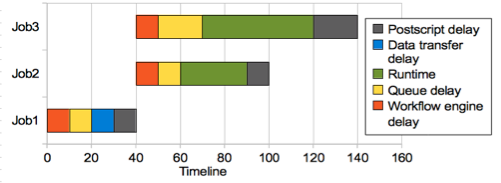
\includegraphics[width=0.5\textwidth]{figures/model/overhead_timeline.pdf}
    \caption{The Timeline of an Example Workflow}
    \label{fig:model_overhead_timeline}
\end{figure}


\begin{figure}[h!]
	\centering
    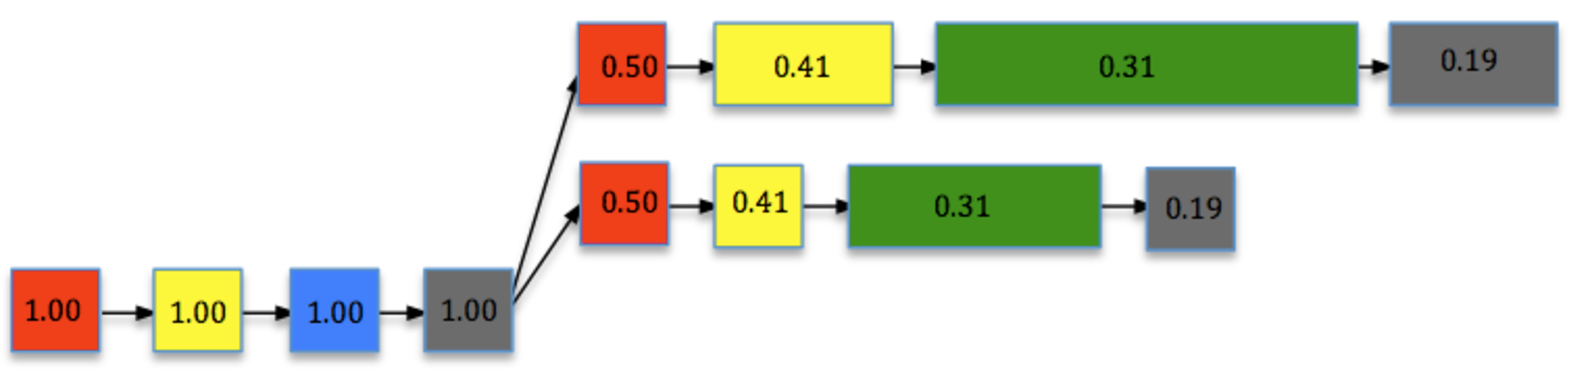
\includegraphics[width=0.5\textwidth]{figures/model/rr.pdf}
    \caption{Reverse Ranking}
    \label{fig:model_rr}
\end{figure}

At $t=0$, job 1, a stage-in job, is released: $queue~delay = 10$, $workflow~engine~delay = 10$, $runtime = 10$, and $postscript~delay = 10$.
At $t=40$, job 3 is released: $workflow~engine~delay = 10$, $queue~delay = 20$, $runtime = 50$, and $postscript~delay = 20$.
At $t=40$, job 2 is released: $workflow~engine~delay = 10$, $queue~delay = 10$, $runtime = 30$, $postscript~delay = 10$. 

%We show how to calculate the cumulative overheads:
 
%For $Sum$:
%$Sum(runtime)=50+30=80$. It contains the time slots of [60, 90] and [70, 120]. 
%$Sum(queue~delay)=10+20+10=40$. It contains [10, 20], [50, 70] and [50, 60]. 
%$Sum(workflow~engine~delay)=10+10+10=30$. It contains [0,10], [40, 50] and [40, 50]. 
%$Sum(postscript~delay)=10+20+10=40$. It contains [30, 40], [90, 100] and [120, 140]. 
%$Sum(data~transfer~delay)=10$. It contains [20, 30].

%For $PJ$:
%$PJ(runtime)=50+30-20=60$. It contains [60, 120].
%$PJ(queue~delay)=10+20+10-10=30$. It contains [10, 20] and [50, 70].
%$PJ(workflow~engine~delay)=10+10+10-10=20$. It contains [0, 10] and [40, 50].
%$PJ(postscript~delay)=10+20+10=40$. It contains [30, 40], [90, 100] and [120, 140].
%$PJ(data~transfer~delay)=10$. It contains [20, 30].

%For $EP$: 
%$EP(runtime)=50+30-20-10-10=40$. It contains [70, 90] and [100, 120].
%$EP(queue~delay)=10+20+10-10-10=20$. It contains [10, 20] and [50, 60]. 
%$EP(workflow~engine~delay)=10+10+10-10=20$. It contains [0, 10] and [40, 50]. 
%$EP(postscript~delay)=10+20+10-10=30$. It contains [30, 40] and  [120,140]. 
%$EP(data~transfer~delay)=10$. It contains [20, 30].

%$RR(runtime)=50\times 0.31+30\times 0.31=24.8$.
%$RR(queue~delay)=10\times 1.00+10\times 0.41+10\times 0.41=18.2$.
%$RR(workflow~engine~delay)=10\times 1.00+10\times 0.50+10\times 0.50=20$.
%$RR(postscript~delay)=10\times 1.00+10\times 0.19+20\times 0.19=15.7$.
%$RR(data~transfer~delay)=10\times 1.00=10$.

In calculating the cumulative runtime, we do not include the runtime of stage-in jobs because we have already classified it as data transfer delay. The overall makespan for this example workflow is 140. Table~\ref{tab:model_percentage_overhead} shows the percentage of overheads and job runtime over makespan.  

\begin{table}[h!]
\caption{Percentage of Overheads and Runtime}
\label{tab:model_percentage_overhead}
\centering
\begin{tabular}{lrrrr}
\hline
Percentage & Sum & PJ & EP &RR\\

\hline

runtime & 57.14\% & 42.86\% & 28.57\% &17.71\% \\
queue delay & 28.57\% &21.43\% &14.29\% &13.00\% \\
workflow engine delay & 21.43\% &14.29\%& 14.29\% &14.29\%\\
postscript delay & 28.57\% & 28.57\% & 21.43\% & 11.21\% \\
data transfer delay & 7.14\% & 7.14\% & 7.14\% & 7.14\% \\
sum & 142.86\% & 114.29\% & 85.71\% & 63.36\%\\
\hline
\end{tabular}
\end{table} 


In Table~\ref{tab:model_percentage_overhead}, we can conclude that the sum of $Sum$ is larger than makespan and smaller than makespan$\times$(number of resources) because it does not count the overlap at all. $PJ$ is larger than makespan since the overlap between more than two types of overheads may be counted twice or more. $EP$ is smaller than makespan since some overlap between more than two types of overheads may not be counted.  $RR$ shows how intensively these overheads and computational activities are connected to each other. 

\subsection{Experiments and Evaluations}

We examined the overhead distributions of a wide range of workflows in our experiments . These workflows were run on distributed platforms including clouds, grids and dedicated clusters. 
On clouds, virtual machines were provisioned and then the required services (such as file transfer services) were deployed. 
We examined two clouds: Amazon EC2 \cite{AmazonEC2}  and FutureGrid \cite{FutureGrid}. Amazon EC2 is a commercial, public cloud that is been widely used in distributed computing. 
We examined the overhead distributions of a widely used astronomy workflow called Montage \cite{Berriman2004} that is used to construct large image mosaics of the sky. Montage was run on FutureGrid \cite{FutureGrid}. FutureGrid is a distributed, high-performance testbed that provides scientists with a set of computing resources to develop parallel, grid, and cloud applications. 
%Should be included in final defense
\subsection{Relationship between Overhead Metrics and Overall Performance}

In this section, we aim to investigate the relationship between the overhead metrics that we proposed and the overall performance of popular workflow restructuring techniques. Among them, task clustering \cite{Singh2008} is a technique that increases the computational granularity of tasks by merging small tasks together into a clustered job, reducing the impact of the queue wait time and also the makespan of the workflow. Data or job throttling \cite{Humphrey2008} limits the amount of parallel data transfer to avoid overloading supporting services such as data servers. Throttling is especially useful for unbalanced workflows in which one task might be idle while waiting for data to arrive. The aim of throttling is to appropriately regulate the rate of data transfers between the workflow tasks via data transfer servers by ways of restricting the data connections, data threads or data transfer jobs. Provisioning tools often deploy pilot jobs as placeholders for the execution of application jobs. Since a placeholder can allow multiple application jobs to execute during its lifetime, some job scheduling overheads can be reduced. 

\textbf{How Task Clustering Reduces Overheads}

In the following sections, we use a Montage workflow to show how different optimization methods improve overall performance. Many workflows are composed of thousands of fine computational granularity tasks. Task clustering is a technique that increases the computational granularity of tasks by merging small jobs together into a clustered job, reducing the impact of the queue wait time and minimizing the makespan of the workflow. Table 4.2 compares the overheads and runtime of the Montage workflow. We can conclude that with clustering, although the average overheads do not change much, the cumulative overheads decrease greatly due to the decreased number of jobs. With clustering, the makespan has been reduced by 53.3\% by reducing the number of all jobs from 3461 to 104 in this example. Figure 4.5 shows the percentage of workflow overheads and runtime. The percentage is calculated by the cumulative overhead ($PJ$, or $EP$) divided by the makespan of workflows. With clustering, the portion of runtime is increased significantly. Figure 4.6 profiles the number of active jobs during execution and it also shows that with clustering the resource utilization is improved significantly. 

\textbf{How Job Throttling Reduces Overheads}

Data or job throttling [13] limits the amount of parallel data transfer to avoid overloading supporting services such as data servers. Throttling is especially useful for unbalanced workflows in which one task might be idle while waiting for data to arrive. The aim of throttling is to appropriately regulate the rate of data transfers between the workflow tasks via data transfer servers by ways of restricting the data connections, data threads or data transfer jobs. Especially on cloud platforms, I/O requests need to go through more layers than a physical cluster; and thereby workflows may suffer a higher overhead from data servers.

In our experiments, the data transfer service is deployed on a virtual machine that is similar to a worker node.  In this section, we evaluate a simple static throttling strategy where the Condor scheduler limits the number of concurrent jobs to be run and thereby restricts the number of parallel I/O requests. There are 32 resources available and we evaluate the cases with throttling parameters that are equal to 24, 16 and 12 in Table 4.3. In the case of 24, the resources are better utilized but the data server is heavily loaded. In the case of 12, the resources are under-utilized even though the data server has more capabilities. In this experiment, both $PJ$ and $EP$ reflect the variation trend of overheads and makespan better than $Sum$. 

Figure 4.7 shows the percentage of workflow overheads and runtime. Figure 4.8 profiles the number of active jobs during execution. Montage is an unbalanced workflow because the three major types of jobs (mProjectPP, mDiffFit, and mBackground) impose a heavy load on the data server while the other jobs in the workflow do not. Figure 4.8 shows that with throttling the maximum number of active jobs is restricted. With limited throttling (reducing threshold from 24 to 16), the data transfer requests are distributed in the timeline more evenly and, as a result, their overhead is reduced. However, with over throttling (reducing threshold from 16 to 12), resources are not fully utilized and thus the makespan is increased. 

\textbf{How Pre-staging Reduces Overheads}

Scientific workflows often consume and produce a large amount of data during execution. Data pre-staging [14] transfers input data before the computational activities are started or even before the workflow is mapped onto resources. Data placement policies distribute data in advance by placing data sets where they may be requested or by replicating data sets to improve runtime performance. In our experiments, because data is already pre-staged, the implementation of the stage-in job is to create a soft link to the data from the workflow’s working directory, making it available to the workflow jobs. Table 4.4 and Figure 4.9 show the cumulative overheads and runtime of the Montage workflows running with and without pre-staging. Looking at the rows for $PJ$ in Table 4.4, we can conclude that pre-staging improves the overall runtime by reducing the data transfer delay. For the case without pre-staging the $EP$ for data transfer delay is zero because it overlaps with the workflow engine delay of another job. Therefore, in this experiment, $PJ$ reflects the variation trend of the makespan more consistently. 

\textbf{How Provisioning Reduces Overheads}

Many of the scientific applications presented here consist of a large number of short-duration tasks whose runtimes are greatly influenced by overheads present in distributed environments. Most of these environments have an execution mode based on batch scheduling where jobs are held in a queue until resources become available to execute them. Such a best-effort model normally imposes heavy overheads in scheduling and queuing. For example, Condor-G [23] uses Globus GRAM [37] to submit jobs to remote clusters. The Globus Toolkit normally has a significant overhead compared to running Condor directly as an intra domain resource and job management system. Provisioning tools often deploy pilot jobs as placeholders for the execution of application jobs. Since a placeholder can allow multiple application jobs to execute during its lifetime, some job scheduling overheads can be reduced. In our experiments, we compared the performance of Condor-G (without provisioning) and Corral (with provisioning). 

Table 4.5 and Figure 4.10 show the percentage of workflow overheads and runtime. The percentage is calculated by the cumulative overhead ($Sum$, $PJ$, or $EP$) divided by the makespan of workflows. Comparing $Sum$, $PJ$ and $EP$, we can conclude that the overheads with provisioning have been reduced significantly because the local scheduler has direct control over the resources without going through Globus. 
